\documentclass[14pt]{beamer}
%\usetheme{Singapore} %Gray with fade at top
%\useoutertheme[subsection=false]{miniframes} %Supppress subsection in header
\useinnertheme{rectangles} %Itemize/Enumerate boxes
\usecolortheme{seagull} %Color theme
\usecolortheme{rose} %Inner color theme

\definecolor{light-gray}{gray}{0.75}
\definecolor{dark-gray}{gray}{0.55}
\setbeamercolor{item}{fg=light-gray}
\setbeamercolor{enumerate item}{fg=dark-gray}

\setbeamertemplate{navigation symbols}{}
%\setbeamertemplate{mini frames}[default]
%\setbeamercovered{dynamics}
\setbeamerfont*{title}{size=\Large,series=\bfseries}
\setbeamerfont*{author}{size=\normalsize,series=\bfseries}
\setbeamerfont*{institute}{size=\normalsize}

\setbeamertemplate{frametitle}{\vspace{.5em}\bfseries\insertframetitle}
\newcommand{\heading}[1]{\noindent \textbf{#1}\\ \vspace{1em}}

\newcommand\Wider[2][3em]{%
\makebox[\linewidth][c]{%
  \begin{minipage}{\dimexpr\textwidth+#1\relax}
  \raggedright#2
  \end{minipage}%
  }%
}


\usepackage{bbding,color,graphicx,verbatim,pbox}

\usepackage[english]{babel}
\usepackage[latin1]{inputenc}
\usepackage[T1]{fontenc}
\usepackage{lmodern}
\usepackage{listings}
\lstset{ % 
  language=R,                % the language of the code 
  basicstyle=\footnotesize\verbatim@font,           % the size of the fonts that are used for the code 
  showspaces=false,               % show spaces adding particular underscores 
  showstringspaces=false,         % underline spaces within strings 
  showtabs=false,                 % show tabs within strings adding particular underscores 
  rulecolor=\color{black},        % if not set, the frame-color may be changed on line-breaks within not-black text (e.g. commens (green here)) 
  tabsize=2,                      % sets default tabsize to 2 spaces 
  breaklines=false,                % sets automatic line breaking 
  breakatwhitespace=false,        % sets if automatic breaks should only happen at whitespace 
  keywordstyle=\color{black},          % keyword style 
  commentstyle=\color{green},       % comment style 
  stringstyle=\color{red},         % string literal style 
  escapeinside={\%*}{*)},            % if you want to add a comment within your code 
  morekeywords={*,...}               % if you want to add more keywords to the set 
} 

\pagecolor{black}
\usepackage{pdfpages}

\usepackage{adjustbox}
\usepackage{tikz}
\usetikzlibrary{shapes,arrows}

\setbeamerfont{title}{size=\Huge,series=\bfseries}
\title{\textcolor{white}{Crowdsourcing with MTurkR}}

\author[]{\textcolor{white}{Thomas J. Leeper}}
\institute[]{
  \textcolor{white}{{\small Department of Political Science, \hspace{0.5em}\raisebox{-0.25em}{
\includegraphics[height=2em]{logo}}}\\
  \vspace{2em}
  {\bfseries Twitter: \href{http://www.twitter.com/thosjleeper}{@thosjleeper}\\
  GitHub:  \href{http://www.github.com/leeper}{leeper}\\
  \href{mailto:thosjleeper@gmail.com}{thosjleeper@gmail.com}}}
}

\date[]{}

\begin{document}

% 15 slides in 5 minutes, where each slide is shown for exactly 20 seconds

% 1
\bgroup
\setbeamercolor{background canvas}{bg=black!80!blue}
\frame{\titlepage}
\egroup

% 2
\begin{frame}[fragile]
\textbf{Imagine we have some data\dots}
\small
\begin{verbatim}
   gender  var1  var2   first       last      image
1  female   0.5     1    sara     annala  img94.jpg
2    male   0.6     3  julius    haataja  img69.jpg
3    male   1.2     2    ross      meyer  img32.jpg
4  female   0.3     1   sarah      lahti  img96.jpg
5  female   1.1     5     ada       park  img24.jpg
6  female   0.9     2    joan  hernandez  img92.jpg
7  female   0.4     1   sofia   korhonen  img87.jpg
8  female   0.1     3   helle     kivela  img52.jpg
9    male   1.8     4  kasper    johnson  img17.jpg
10   male   0.6     2    dirk      luoma  img62.jpg
\end{verbatim}

{\normalsize\raggedleft\textbf{\dots but how do we analyze an \textit{image} variable?}}
\end{frame}


% 3
{
\setbeamercolor{background canvas}{bg=}
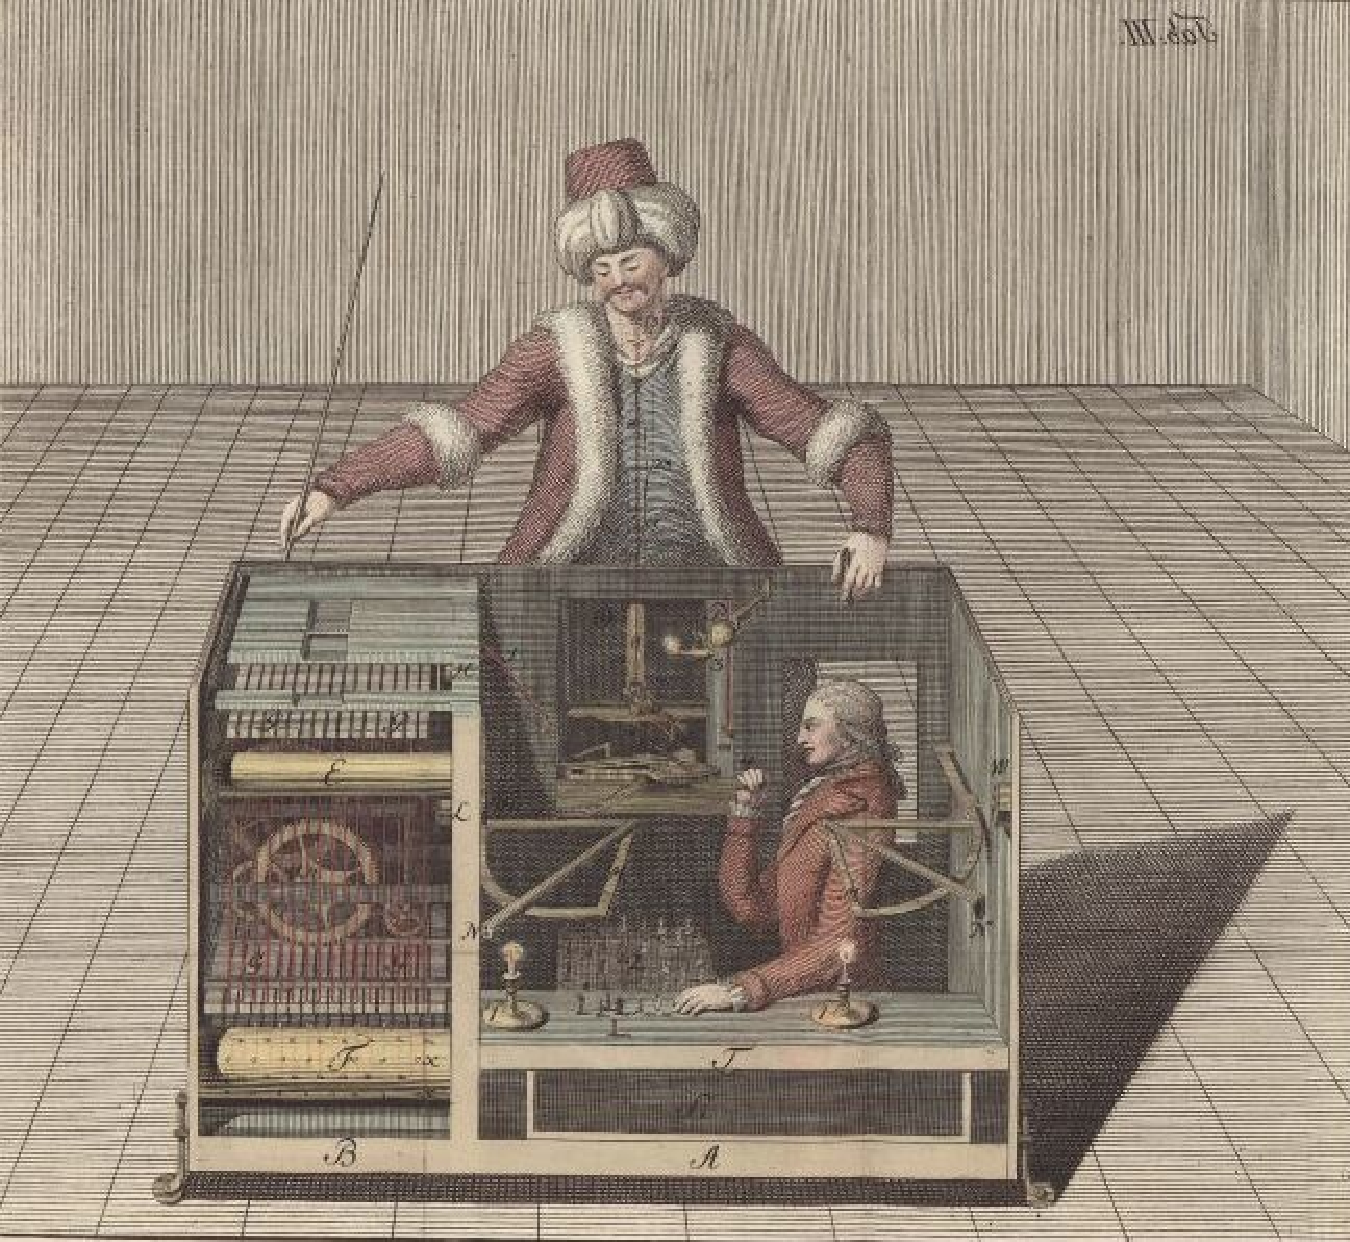
\includepdf{turk.pdf}
}

% 4
\bgroup
\setbeamercolor{background canvas}{bg=black}
\begin{frame}[fragile]
\large
\Wider[2em]{
\begin{center}
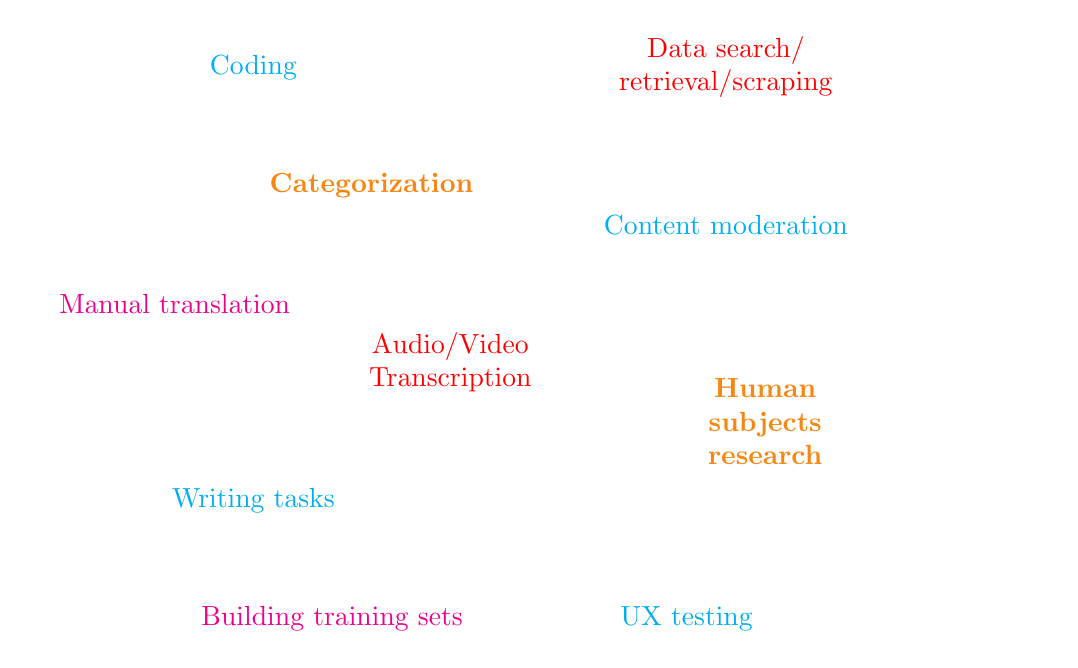
\begin{tikzpicture}
    \node[align=center, text width=3.5cm] at (0,6) () {\textcolor{cyan}{Coding}};
    \node[align=center, text width=3.5cm] at (-1,3) () {\textcolor{magenta}{Manual translation}};
    \node[align=center, text width=3.5cm] at (0,0.5) () {\textcolor{cyan}{Writing tasks}};
    \node[align=center, text width=3.5cm] at (5.5,-1) () {\textcolor{cyan}{UX testing}};
    \node[align=center, text width=3.5cm] at (6,4) () {\textcolor{cyan}{Content moderation}};
    \node[align=center, text width=3.5cm] at (2.5,2.25) () {\textcolor{red}{Audio/Video Transcription}};
    \node[align=center, text width=5cm] at (6,6) () {\textcolor{red}{Data search/\\retrieval/scraping}};
    \node[align=center, text width=3.5cm] at (1,-1) () {\textcolor{magenta}{Building training sets}};
    \node[align=center, text width=3.5cm] at (1.5,4.5) () {\textcolor{yellow!50!red}{\textbf{Categorization}}};
    \node[align=center, text width=7cm] at (6.5,1.5) () {\textcolor{yellow!50!red}{\textbf{Human\\subjects\\research}}};
\end{tikzpicture}
\end{center}
}
\end{frame}
}

% 5
\begin{frame}[fragile]
\large
\begin{center}
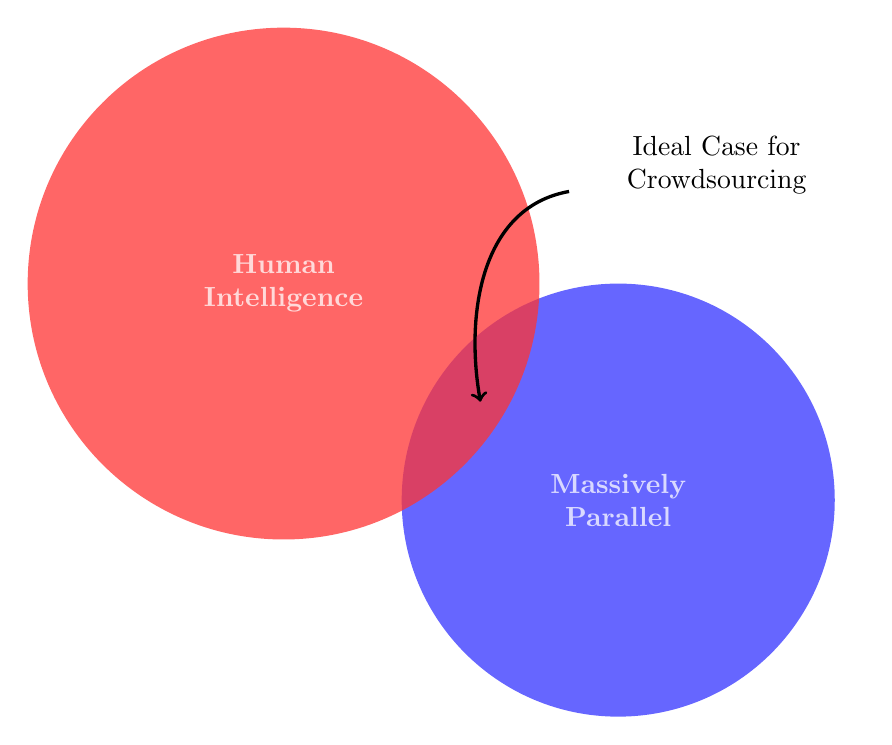
\begin{tikzpicture}
    \fill[blue!80,opacity=0.75] (4.25,0.25) circle (2.75cm) 
        node[text=white, align=center, text width=3cm] {\textbf{Massively\\ Parallel}};
    \fill[red!80,opacity=0.75] (0,3) circle (3.25cm) 
        node[text=white, align=center, text width=3cm] {\textbf{Human\\ Intelligence}};
    \node[align=center, text width=3.5cm] at (5.5,4.5) (c) {Ideal Case for\\ Crowdsourcing};
    \draw[->,very thick] (c) to [out = 190, in = 100, looseness = 1] (2.5,1.5);
% use-cases: scraping, coding, human subjects research
% crowdsourcing is a form of parallel computing
\end{tikzpicture}
\end{center}
\end{frame}


% 6
\begin{frame}[fragile]
\vspace{1em}
% Define block styles
\tikzstyle{decision} = [diamond, draw, fill=blue!20, 
    text width=4.5em, text badly centered, node distance=3cm, inner sep=0pt]
\tikzstyle{block} = [rectangle, draw, fill=blue!20, draw=none,
    text width=2cm, text centered, rounded corners, minimum height=4em]
\tikzstyle{line} = [draw, -latex', line width=1.5pt, color=gray!95]
\tikzstyle{cloud} = [draw, ellipse,fill=blue!20, draw=none, minimum height=2em]

\begin{adjustbox}{max totalsize={\textwidth}{\textheight},center}
\begin{tikzpicture}[scale=0.5,node distance = 2cm, auto]
    % Place nodes
    \node [block, text=white, fill=blue!65, minimum width=3cm, text width=4cm] (init) {\Large\textbf{Data Need}};
    \node [block, below of=init, node distance=5cm, minimum width=3cm, text width=5cm, fill=gray!15] (design) {\Large\textbf{Design Data Entry Form}};
    	Register HITType
    	};
    \node [block, below of=design, node distance=5cm, minimum width=4cm, text width=4cm] (createhit) {
    	\Large \textbf{Create HIT(s)}
    	};
    \node [cloud, right of=createhit, node distance=6cm, fill=red!20] (assignment3) {Assignment};
    \node [cloud, above of=assignment3, node distance=1cm, fill=red!20] (assignment2) {Assignment};
    \node [cloud, above of=assignment2, node distance=1cm, fill=red!20] (assignment1) {Assignment};
    \node [cloud, below of=assignment3, node distance=1cm, fill=red!20] (assignment4) {Assignment};
    \node [cloud, below of=assignment4, node distance=1cm, fill=red!20] (assignment5) {Assignment};
    \node [block, right of=assignment3, node distance=6cm, minimum width=3cm, text width=3cm] (review) {\Large \textbf{Review}};
    \node [block, above of=review, node distance=10cm, text=white, fill=blue!65, minimum width=3cm, text width=4cm] (analyze) {\Large\textbf{Analyze data}};
    
    \node [left of=init, node distance=6cm, align=left] (R) {\Large\textbf{R}};
    \node [below of=R, node distance=5cm, align=left] (html) {\Large\textbf{HTML}};
    \node [below of=html, node distance=5cm, align=left] {\Large\textbf{MTurk}};
    
    %     % Draw edges
    \path [line] (init) -- (design);
    \draw [line] (design) to [out=270,in=90] (createhit);
    \draw [line] (createhit) to [out=20, in=180] (assignment1);
    \draw [line] (createhit) to [out=10, in=180] (assignment2);
    \draw [line] (createhit) to [out=0, in=180] (assignment3);
    \draw [line] (createhit) to [out=350, in=180] (assignment4);
    \draw [line] (createhit) to [out=340, in=180] (assignment5);
    \draw [line] (assignment1) to [out=0, in=160] (review);
    \draw [line] (assignment2) to [out=0, in=170] (review);
    \draw [line] (assignment3) to [out=0, in=180] (review);
    \draw [line] (assignment4) to [out=0, in=190] (review);
    \draw [line] (assignment5) to [out=0, in=200] (review);
    \path [line] (review) -- (analyze);
\end{tikzpicture}
\end{adjustbox}

\end{frame}

% 7
\begin{frame}
\includegraphics[width=\textwidth]{screencap}
\end{frame}


% 8
\bgroup
\setbeamercolor{background canvas}{bg=black}
\begin{frame}
\Wider[2em]{\small\vspace{1em}
{\color{white}\texttt{\noindent \# set API keys in environment variables\\
\vspace{1em}
library("MTurkR")\\
\vspace{1em}
BulkCreateFromURLs(\\
\hspace{0.5em}    url = paste0("https://example.com/",1:10,".html"),\\    
\vspace{1em}
\hspace{0.5em}    title = "Image Categorization",\\
\hspace{0.5em}    description = "Describe contents of an image",\\
\hspace{0.5em}    keywords = "categorization, image",\\
\hspace{0.5em}    reward = .01,\\
\hspace{0.5em}    duration = seconds(minutes = 5),\\
\vspace{1em}
\hspace{0.5em}    annotation = "My Project",\\
\hspace{0.5em}    expiration = seconds(days = 4),\\
\hspace{0.5em}    auto.approval.delay = seconds(days = 1)\\
)
}}}
\end{frame}
\egroup

% 9: `GetAssignments`
\begin{frame}[fragile]
\textbf{Get back a data.frame:}\\
\vspace{2em}
\texttt{GetAssignments(annotation = "My Project")}\\
\vspace{2em}
\def\arraystretch{1.5}
\begin{tabular}{rl}
The image coding task with & \textbf{27,500 images}\\
                      took & \textbf{225 workers}\\
                     about & \textbf{75 minutes}\\
                  and cost & \textbf{\$412.50}\\
\end{tabular}

\vspace{2em}
{\small \textcolor{gray}{Pay workers with:\\ \texttt{ApproveAssignments(annotation = "My Project")}}}
\end{frame}

% 10
\bgroup
\setbeamercolor{background canvas}{bg=black}
\begin{frame}
\Wider[1em]{\vspace{1em}
{\color{white}\texttt{\noindent a = GenerateHTMLQuestion(file = "hit.html")\\
\vspace{1em}
hit = CreateHIT(\\
\hspace{0.5em}  title = "Short Survey",\\
\hspace{0.5em}  description = "5 question survey",\\
\hspace{0.5em}  keywords = "survey, questionnaire",\\
\hspace{0.5em}  duration = seconds(hours = 1)\\
\hspace{0.5em}  reward = .10,\\
\vspace{1em}
\hspace{0.5em}  assignments = 5000,\\
\hspace{0.5em}  expiration = seconds(days = 4),\\
\hspace{0.5em}  question = a\$string,\\
)
}}}
\end{frame}

% 11
\begin{frame}
\Wider[1em]{\vspace{1em}
{\color{white}\texttt{\noindent GetHIT(hit\$HITId)\\
\vspace{1em}
ExtendHIT(hit\$HITId,\\
\hspace{0.5em}  add.assignments = 500)\\
\hspace{0.5em}  add.seconds = seconds(days = 1)\\
)\\
\vspace{1em}
ExpireHIT(hit\$HITId)\\
\vspace{1em}
ChangeHITType(hit\$HITId,\\
\hspace{0.5em}  title = "New, better title",\\
\hspace{0.5em}  reward = 5.00\\
)
}}}
\end{frame}

%\begin{frame}
%\Wider[1em]{\vspace{1em}
%{\color{white}\texttt{\noindent a = GetAssignments(hit = hit)\\
%\vspace{0.5em}
%ContactWorkers(\\
%\hspace{0.5em}  subjects = "Hello again!",\\
%\hspace{0.5em}  msgs = "Stuff I want to say to you",\\
%\hspace{0.5em}  workers = a\$WorkerId\\
%)\\
%\vspace{0.5em}
%GrantBonus(\\
%\hspace{0.5em}  workers = a\$WorkerId,\\
%\hspace{0.5em}  assignments = a\$AssignmentId,\\
%\hspace{0.5em}  amount = 0.50,\\
%\hspace{0.5em}  reasons = "Nice work!"\\
%)
%}}}
%\end{frame}

\egroup


% 12: Management features
\bgroup
\setbeamercolor{background canvas}{bg=black!80!blue}
\begin{frame}
    \frametitle{\textcolor{white}{Advanced Features}}
    \large
    \centering
    \def\arraystretch{2.5}
    \begin{tabular}{lcl}
    \pbox{9em}{\textcolor{white}{Choose who works\newline for you}} & \textcolor{white}{$\Rightarrow$} & \pbox{9em}{\textcolor{white}{Qualifications\newline and tests}}\\
    \pbox{9em}{\textcolor{white}{Monitor HITs}} & \textcolor{white}{$\Rightarrow$} & \pbox{9em}{\textcolor{white}{Notifications}}\\
    \pbox{9em}{\textcolor{white}{Sanction and reward\newline workers}} & \textcolor{white}{$\Rightarrow$} & \pbox{9em}{\textcolor{white}{Qualifications, bonuses, and blocks}}\\
    \pbox{9em}{\textcolor{white}{Automatic review}} & \textcolor{white}{$\Rightarrow$} & \pbox{9em}{\textcolor{white}{Review Policies}}\\
    \end{tabular}
\end{frame}
\egroup

% 13
\begin{frame}[fragile]
\frametitle{Anatomy of an MTurkR App}
% Define block styles
\begin{center}
    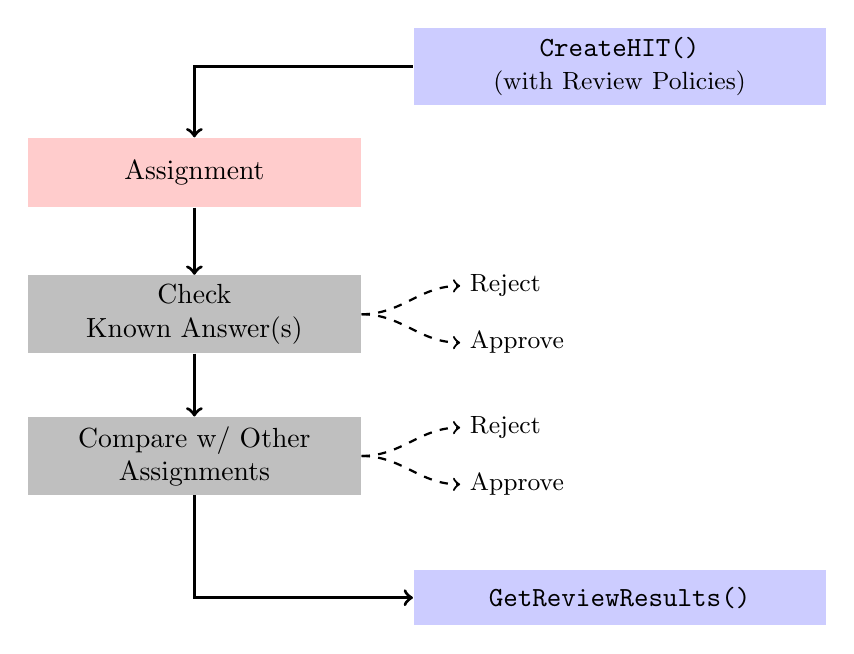
\begin{tikzpicture}[scale=0.9]
    \node[fill=red!20, text width=4cm, minimum height=2.5em, align=center] at (0,6) (assign) {Assignment};
    \node[fill=blue!20, text width=5cm, minimum height=2em, align=center] at (6,7.5) (create) {\texttt{CreateHIT()}\\ {\small (with Review Policies)}};
    \draw[->, very thick] (create) -| (assign);
    \node[fill=gray!50, text width=4cm, align=center] at (0,4) (known) {Check\\ Known Answer(s)};
    \draw[->, very thick] (assign) to (known);
    \node [text width = 2cm] at (5,4.4) (reject1) {\small Reject};
    \node [text width = 2cm] at (5,3.6) (approve1) {\small Approve};
    \draw[->, dashed, thick] (known) to [out=0, in=180] (approve1);
    \draw[->, dashed, thick] (known) to [out=0, in=180] (reject1);
    \node[fill=gray!50, text width=4cm, align=center] at (0,2) (hit) {Compare w/ Other Assignments};
    \draw[->, very thick] (known) to (hit);
    \node [text width = 2cm] at (5,2.4) (reject2) {\small Reject};
    \node [text width = 2cm] at (5,1.6) (approve2) {\small Approve};
    \draw[->, dashed, thick] (hit) to [out=0, in=180] (approve2);
    \draw[->, dashed, thick] (hit) to [out=0, in=180] (reject2);
    \node[fill=blue!20, text width=5cm, minimum height=2em, align=center] at (6,0) (results) {\texttt{GetReviewResults()}};
    \draw[->, very thick] (hit) |- (results);
    \end{tikzpicture}
\end{center}
\end{frame}

% 14
\begin{frame}
    \frametitle{What's next?}
    \begin{columns}
        \begin{column}{.5\linewidth}
          \begin{enumerate}\itemsep2em
          \item \textbf{Packages for more crowdsourcing platforms}\\
              \begin{itemize}
              \item Common interface?
              \end{itemize}
          \item \textbf{HIT templates}
          \item \textbf{Performance improvements}
          \end{enumerate}
        \end{column}
        \begin{column}{.5\linewidth}
            \includegraphics[width=\textwidth]{mturk}
            \vspace{2em}
            
            \includegraphics[width=\textwidth]{microworkers}
            \vspace{2em}
                        
            \includegraphics[width=\textwidth]{crowdflower}
            \vspace{2em}
                        
            \includegraphics[width=\textwidth]{prolificacademic}
        \end{column}
    \end{columns}
\end{frame}





% 15
\bgroup
\setbeamercolor{background canvas}{bg=black}
\begin{frame}
    \vspace{1em}
    {\color{white}\texttt{\noindent \# Start Crowdsourcing\\
    \vspace{1.5em}
    \# CRAN\\
    install.packages("MTurkR")\\
    \vspace{1.5em}
    \# GitHub\\
    install\_github("leeper/MTurkR")\\
    \vspace{1.5em}
    \# Questions?\\
    \# \href{mailto:thosjleeper@gmail.com}{thosjleeper@gmail.com}\\
    \# \url{https://github.com/leeper/MTurkR/wiki} }}
\end{frame}
\egroup


\end{document}